%!TEX root = dissertation.tex
%%%%%%%%%%%%%%%%%%%%%%%%%%%%%%%%%%%%%%%%%%%%%%%%%%%%%%%%%%%%%%%%%%%%%%%%%%%%%%%%
\chapter{Mobile Core Networks}



%%%%%%%%%%%%%%%%%%%%%%%%%%%%%%%%%%%%%%%%%%%%%%%%%%%%%%%%%%%%%%%%%%%%%%%%%%%%%%%%
\section{Architecture of GSM derived mobile networks}



%%%%%%%%%%%%%%%%%%%%%%%%%%%%%%%%%%%%%%%%%%%%%%%%%%%%%%%%%%%%%%%%%%%%%%%%%%%%%%%%
\section{Traffic Characteristics}



%%%%%%%%%%%%%%%%%%%%%%%%%%%%%%%%%%%%%%%%%%%%%%%%%%%%%%%%%%%%%%%%%%%%%%%%%%%%%%%%
\section{Control Plane and Signaling Analysis}
\subsection{Traffic Transport}
\subsubsection{PDP Contexts and LTE Bearers}
\subsection{Control Messaging Protocols}
\subsection{Control Messaging Causes}



%%%%%%%%%%%%%%%%%%%%%%%%%%%%%%%%%%%%%%%%%%%%%%%%%%%%%%%%%%%%%%%%%%%%%%%%%%%%%%%%
\section{Signaling Load Observations}



%%%%%%%%%%%%%%%%%%%%%%%%%%%%%%%%%%%%%%%%%%%%%%%%%%%%%%%%%%%%%%%%%%%%%%%%%%%%%%%%
\section{CoNEXT2012 Core Signaling INLET}


%%%%%%%%%%%%%%%%%%%%%%%%%%%%%%%%%%%%%%%%%%%%%%%%%%%%%%%%%%%%%%%%%%%%%%%%%%%%%%%%
\section{Introduction}
\label{sec:introduction-CONEXT}

Given its roots as a research network and its growing pervasiveness over the last forty years, it is understandable that research on the Internet covers all parts of the network from applications to access to the core, and has been going on ever since what could be considered prehistoric times of the Net. The state of research on mobile cellular networks such as 3G is lean in comparison. Mobile networks providing Internet access have not been around for too long, and still are not available in all parts of the world. Furthermore, most research focuses on user-oriented metrics such as traffic statistics and mobility patterns, or takes into account the radio part of the network only. Little has been published about activity within the core network, and yet less about signaling.

Given how limited spectral resources on the radio interface are, it might not seem obvious to think about signaling load in the network. Yet, there have been situations where the core network unintentionally has been flooded with signaling, taking down user-plane connectivity on the way, despite small amounts of actual user traffic being transported \cite{lt2012docostorm, it2011birdandroid}. 

The adverse effects of state-keeping in network devices have been known to, e.g.,  Internet users running BitTorrent across low-end home routers as of the early 2000s. In \ac{UMTS} mobile networks, the networking hardware is vastly more powerful, but the control plane tasks are vastly more complex than port and network translation as well, namely carrying and routing IP and voice traffic, user mobility, \ac{AAA} and so on. Many specialized protocols are involved to communicate intents and states in the network. This causes processing overhead, additional traffic on network paths, and increases the number of states to be held in memory on the core network nodes. Therefore, in scenarios such as the ones mentioned above, radio access is not the bottleneck to connectivity any more, but signaling is.

The inherent complexity of signaling in mobile cellular networks is easily missed by programmers who do not or cannot know that their applications will run over such wireless links, and probably would not expect it from a network that pretends to transparently carry IP. What furthers this problem is the lack of literature on the theoretical and practical sides of these issues.

This apparent lack is due to a number of reasons. First, gaining sufficiently intimate knowledge on the huge corpus of \ac{3GPP} Technical Specifications %\ac{TS}
is a laborious task. Second, to come up with lower-layer measurements requires physical access to the core network infrastructure and suitable measurement equipment. Also, much of the data is commercially and privacy-sensitive, and cannot be published without extensive sanitizing.

The purpose of this paper will therefore be to give a 3G tunnel management primer, introducing the relevant \acs{GPRS}/\acs{UMTS} network structure and the involved control plane protocols with a special focus on the \ac{GTP}, which is probably the most prevalent. % We discuss how much overhead is put on the network through \ac{GTP} in a typical user traffic scenario.
Furthermore, we share our first insights into one practical aspect of the signaling process, the \ac{GTP} tunnel management procedures. Using a week long data set from an Austrian mobile operator recorded at the Gn interface between the \ac{SGSN} and \ac{GGSN}, % by the \ac{METAWIN} measurement infrastructure from the FTW, 
we take a look at \ac{PDP} Context durations, i.e. the time a \ac{PDP} Context is established and held, argue how this influences the load on the network, and evaluate the data by device types and operating systems.

Our measurement data backs up a number of straightforward assumptions on the behavior of different device and operating system types, but also reveals some remarkable differences in tunnel characteristics.\\

The rest of the paper is structured as follows. Section \ref{sec:relwork} discusses relevant work in the field. Section \ref{sec:gtp} introduces \ac{UMTS} as well as \ac{GTP} basics and protocol details relevant to core signaling. Chapter \ref{sec:darwin} gives an overview on the \acs{METAWIN} data acquisition platform. Chapter \ref{sec:evaluations-CONEXT} evaluates our data set, and Chapter \ref{sec:conclusion-CONEXT} concludes the paper and gives an outlook to future endeavors.


%Traditionally, mobile network performance evaluation is either done by active probing through the handset, or, in case of passive measurements, with a heavy focus on radio performance. In this paper, we instead Stake an initial look on control plane performance characteristics in mobile core networks. Our focus lies on evaluating GTP Tunnel Management signaling messages on the path between SGSN and GGSN and the overhead imposed on user plane traffic. Therefore, we make an effort to correlate PDP Context durations to device specific parameters such as device class, e.g., dongles or smartphones, or operating system. From the context duration we can then estimate the signaling overhead each device burdens on the core network.



%%%%%%%%%%%%%%%%%%%%%%%%%%%%%%%%%%%%%%%%%%%%%%%%%%%%%%%%%%%%%%%%%%%%%%%%%%%%%%%%
\section{Related Work}
\label{sec:relwork}

%The first and foremost literature in any control plane protocol investigations are the specifications itself.
%3gpp GSM/UMTS/LTE specs on GPRS (also applicable for UMTS data transport) \cite{3gpp23060} and GTP \cite{3gpp29060}


Recently, stories about signaling storms and overloaded control planes in mobile networks reached popular news media \cite{it2011birdandroid, lt2012docostorm}. These stories blame a specific combination mobile device type, operating system and application to cause excessive amounts of signaling in the network. The Android version of the popular casual game ``Angry Birds'' is a free download, and  uses regularly refreshed advertisements to achieve some form of financial compensation for the authors. Now imagine a large amount of devices setting up and tearing down data connections only to retrieve new ads and therefore causing tens of control plane messages on each retrieval, which could strain the signaling-heavy structure of current networks. 

The dynamics behind such events are worth investigating, and some work has already been done by several publications. While these touch parts of the areas tackled in this paper to some degree, we think that the combination of the focus on core signaling, PDP Context durations, and investigating the influence of devices on these are genuine contributions of our work.

When control plane aspects of mobile networks are considered, the investigation usually focusses on the radio interface and \ac{RRC} signaling, but pays little attention to aspects in the core network. A paper on cross-layer interaction in mobile cellular networks falls into this category \cite{qian2011profiling}, discussing interaction, e.g., between the application layer and the \ac{RRC} (such as seen in the ``Angry Birds'' case) and its consequences for device energy consumption and radio channel allocation efficiency. The authors argue that there is much room for improvement in this area, and propose some enhancements.

In \cite{lee2007detection}, mobile network traces are used to simulate a malicious signaling storm by transmitting low-volume user plane traffic with inter-departure times slightly larger than the transition timers in the \ac{RRC} state machines. This constantly causes signaling to occur. The authors propose tools to detect this, and discuss possible scales of this type of denial-of-service attack.

Recent publications concerning device differentiation in mobile networks usually either focus on the user traffic dynamics \cite{shafiq2011characterizing}, or on mobility and the temporal and spatial variations of user traffic resource usage  \cite{paul2011understanding}.

In 2006, Svoboda et al. \cite{svoboda2006composition} conducted a core network measurement study of various user traffic related patterns, and also provided an initial insight into \ac{PDP} context activity and durations. Finally, a recent publication \cite{he2012panoramic} provides an investigation probably closest to our approach, however again aimed at \ac{RRC} signaling on the Iu-PS link and not at \ac{GTP} signaling at the Gn path (both of which somewhat intertwined however). The authors classify their evaluations based on device model and vendor and on the application type, and find that different devices have strongly different \ac{RRC} characteristics, which could possibly also have an impact on \ac{GTP} signaling.


%A Panoramic View of 3G Data/Control-Plane Traffic: Mobile Device Perspective He \cite{he2012panoramic}

%In \cite{shafiq2011characterizing} Shafiq et al. focus solely on the user traffic dynamics of devices in mobile networks, but one can already observe that classification by device type is an interesting option for mobile networks. Another large scale user traffic dynamic study was conducted in \cite{paul2011understanding} but also solely focuses on user plane aspects of resource usage.

%Characterizing and Modeling Internet Traffic Dynamics of Cellular Devices Shafiq \cite{shafiq2011characterizing} 
%Understanding Traffic Dynamics in Cellular Data Networks Paul \cite{paul2011understanding}
%Profiling resource usage for mobile applications: a cross-layer approach Qian \cite{qian2011profiling}
% Not really needed: An Untold Story of Middleboxes in Cellular Networks Wang \cite{wang2011untold}
% Auch unnötig: Cellular data network infrastructure characterization and implication on mobile content placement Xu\cite{Xu:2011:CDN:2007116.2007149}
% 		Regarding investigations of network infrastructure we again see an user network layer centric approach in \cite{Xu:2011:CDN:2007116.2007149}
% Not accepted! Analyzing 3G Control-Plane Signaling Overhead from a Data-Plane Perspective Qian \cite{qian2012radiosigoh}
% nur in die darwin section: Traffic monitoring and analysis in 3G networks: lessons learned from the METAWIN project \cite{ricciato2006traffic}
%Composition of GPRS, UMTS traffic: snapshots from a live network Svoboda \cite{svoboda2006composition}
%On the detection of signaling DoS attacks on 3G wireless networks Lee \cite{lee2007detection}
%A Comparison Between One-way Delays in Operating HSPA and LTE Networks \cite{laner2012delaycomparison}


%%%%%%%%%%%%%%%%%%%%%%%%%%%%%%%%%%%%%%%%%%%%%%%%%%%%%%%%%%%%%%%%%%%%%%%%%%%%%%%%
\section{GPRS and Tunnel Management}
\label{sec:gtp}
\acresetall
This section starts with a primer on cellular data network basics, and then moves on to describe relevant details of \ac{GTP}, the tunneling protocol under investigation.

%---
%NSAPI {0;15} Integer
%linked NSAPI: indicates the NSAPI assigned to any one of the already activated PDP contexts for this address/phone ("foreign key"?)


\subsection{\acs{GPRS} Fundamentals}

Before diving into specifics of \ac{GTP} messaging, we give a short overview on the packet switched domain of an \ac{UMTS} network. This domain is closely related to the \ac{GPRS} part introduced for \acs{GSM}. \ac{UMTS}, first defined by the \ac{3GPP} in Release 99, focuses its improvements over \ac{GSM} mostly on the radio aspects, while keeping the core network \ac{GPRS} architecture intact at large. \ac{3GPP} \ac{TS} 23.060 \cite{3gpp23060} defines the basic aspects involving \ac{GPRS} protocols and its system architecture. \ac{TS} 29.060 \cite{3gpp29060} describes the specifics of \ac{GTP} flowing across the Gn and Gp interfaces which forms the basis for our work.


\begin{figure*}
\centering
\includegraphics[width=0.7\textwidth]{images/umts-network.pdf}
\caption{Typical simplified setup of the packet switched domain in an \acs{UMTS} network including a METAWIN monitoring probe.}
\label{fig:umtsnetwork}
\end{figure*}



As shown in Figure \ref{fig:umtsnetwork}, user traffic originating at any \ac{MS} connected to the radio network flows through one of the Node Bs, providing radio connectivity. Multiple Node Bs are aggregated by a \ac{RNC}. Node Bs and \acp{RNC} form the \ac{UTRAN}, which is typically connected by back-haul fiber links to the core network part formed by the \ac{SGSN} and the \ac{GGSN}.

One role of the \ac{SGSN} is as the mobility anchor for mobile devices, and it is the endpoint for \ac{RRC}-based signaling and the \ac{RAB}. The \ac{GGSN} provides the gateway to the public Internet. The Gn interface connects those two nodes, using the \ac{GTP} protocol to exchange user as well as control plane traffic as seen in the protocol stack in Figure \ref{fig:signallingstack}. \ac{GTP} is further separated into GTP-C, facilitating control message exchange, and GTP-U for transporting user traffic through tunnels.


\begin{figure}
\centering
\includegraphics[width=0.6\columnwidth]{images/signalling-stack.pdf}
\caption{Typical signaling protocol stack at the Gn interface between \ac{SGSN} and \ac{GGSN}.}
\label{fig:signallingstack}
\end{figure}




%%%%%%%%%%%%%%%%%%%%%%%%%%%%%%%%%%%%%%%%%%%%%%%%%%%%%%%%%%%%%%%%%%%%%%%%%%%%%%%%
\subsection{GTP Signaling}


Tunnels are defined in the \ac{SGSN} and \ac{GGSN} in \ac{PDP} Context data structures. These hold various information related to a tunnel, such as the device IP address, \ac{IMSI}, and a tunnel identifier. A tunneling concept is used for user traffic to isolate it from core network control plane traffic and to provide certain \ac{QoS} guarantees to the user traffic. To distinguish multiple \ac{QoS} profiles per device, up to ten additional secondary contexts can be established beyond the primary PDP context, all with different \ac{QoS} allocations. However, secondary contexts are rarely in use today, and any user-plane IP traffic is transported within the primary ``best effort'' tunnel.

As already mentioned, GTP-C signaling is used to administer these contexts. Across the Gn path, it contains procedures for managing data paths, \ac{MS} locations, mobility, and, of course, tunnels. We take a specific look at the last one. \ac{GTP} messages usually come as request-response pairs. Neither part has fixed size, but is rather constructed from a number of \acp{IE} of partially variable length. 

The focus of our work will be the three Tunnel Management message pairs involved in the maintenance of PDP Contexts. These are the \textit{Create, Update,} and \textit{Delete PDP Context Requests} and \textit{Responses}. Each pair, including their causes and possible effects, will be treated in a separate section, with the Create and Delete messages forming the substrate for our investigations presented in this paper.

The variable-length nature of these messages makes evaluating the imposed network signaling load rather difficult. For example, the Create Context Response consists of up to 36 \acp{IE}, some of them mandatory, most either conditional or optional. Including the headers of both the packet and the individual elements, the minimum size (counting only the required bytes of variable length elements) is 52 bytes, while the minimal maximum size with all \acp{IE} present is 307 bytes.

Taking this maximum value we arrive at a naive estimate of the maximum overhead on user traffic imposed by tunnel management signaling in our dataset. The ratio of (tunnel management) signaling traffic to total user plane traffic is a minute $0.10\%$. Therefore, the sheer volume of control plane traffic appears to be non-critical in this setup. We assume thus that the overload problems mentioned above arise rather in areas affected by signaling except for the pure transport of data, such as the memory profile of the states kept in the gateway nodes, the time required to process the large number of information held in the messages, or the imposed latency through several message round trips during transactions. The detailed mechanics of system load could be a field of investigation for future work.




%example GTP tunnel management message flow for one instance
%involved core elements
%overhead calculation through type of information elements involved




%%%%%%%%%%%%%%%%%%%%%%%%%%%%%%%%%%%%%%%%%%%%%%%%%%%%%%%%%%%%%%%%%%%%%%%%%%%%%%%%
\subsubsection{Create Context Messages}
\begin{figure}
\centering
\includegraphics[width=0.8\columnwidth]{images/pdp-context-activation.pdf}
\caption{PDP Context Activation Procedure in a UMTS network.}
\label{fig:pdpcontextactivation}
\end{figure}

Figure \ref{fig:pdpcontextactivation} shows the \textit{PDP Context Activation Procedure} as defined in \cite{3gpp23060}. Some additional \ac{CAMEL} procedures may be involved in the creation but are not of interest in the context of this paper as they are not required. Tunneling messages are usually triggered by other procedures on different interfaces. In the case depicted here, the procedure is initiated by the mobile device through a \ac{RANAP} protocol \textit{Activate PDP Context Request} typically sent when establishing a mobile data connection.

Generally speaking, any Create Request is part of a \textit{GPRS PDP Context Activation} procedure, which can happen under several circumstances, the aforementioned one being the typical, but also during each \textit{Secondary PDP context Activation} procedure for every tunnel beyond the first. When a \ac{GGSN} receives this request from an \ac{SGSN}, it attempts to complete the Context creation. Depending on the outcome, a response is sent back, indicating the success or failure of the operation. Typical failure codes observed in our measurements were either due to incorrect information supplied by the device (``user authentication failed''), due to malformed messages (e.g. ``invalid message format''), or indicated problems or temporary overload in the network (``no resources available'' and ``system failure'').




%%%%%%%%%%%%%%%%%%%%%%%%%%%%%%%%%%%%%%%%%%%%%%%%%%%%%%%%%%%%%%%%%%%%%%%%%%%%%%%%
\subsubsection{Update Context Messages}

The possible causes for an \textit{Update Context Request} are as following.

\begin{itemize}
\item The mobile devices moves between \acp{SGSN}, causing a \textit{GPRS inter-SGSN Routing Area Update} procedure.
\item Parameters belonging to the context such as the assigned \ac{QoS} are altered using the the \textit{PDP Context Modification}.
\item As part of \textit{Context redistribution and load balancing} procedures.
\item The \ac{MS} switches between \ac{UMTS} and \ac{GPRS} access technologies, causing a \textit{Inter-system intra- \\SGSN Update} procedure. Note that the same tunnel can be used regardless of the radio technology.
\item As part of a direct \ac{RNC} to \ac{GGSN} GTP-U tunnel activation procedure, thereby circumventing the \ac{SGSN}. Or, finally, 
\item To activate secondary PDP contexts using the \textit{Secondary PDP Context Activation} as previously described. 
\end{itemize}

By observing Update Context message one could, for example, capture most forms of mobility happening in the network, and get a good picture of correlations between mobility and tunneling characteristics. Additionally, tunnels using \ac{UMTS} and \ac{GPRS} radio technology can be distinguished, which should in theory lead to wholly different pictures, as nowadays GSM/GPRS is either used in older models or feature phones, or in mobile scenarios in rural areas where the larger GSM cells are more prevalent. Both could indicate that the data session will be rather short  due to either clumsy devices or the low throughput rates of \ac{GPRS}.

%%%%%%%%%%%%%%%%%%%%%%%%%%%%%%%%%%%%%%%%%%%%%%%%%%%%%%%%%%%%%%%%%%%%%%%%%%%%%%%%
\subsubsection{Delete Context Messages}

The third type of Tunnel Management messages are the \textit{Delete Context Request} and \textit{Response}, indicating the immediate release of the Context involved. They are part of 

\begin{itemize}
\item The \textit{GPRS Detach} procedure from the \ac{SGSN} to the \ac{GGSN}, when a device completely deactivates its data services.
\item The \textit{GPRS PDP Context Deactivation} procedure from the \ac{SGSN} to the \ac{GGSN}, if only one specific tunnel is to be removed.
\item The \textit{part of PDP Context Deactivation Initiated by GGSN} procedure signaled to the \ac{SGSN}.
\end{itemize}



%can also delete a set of contexts assigned to a single MS



%%%%%%%%%%%%%%%%%%%%%%%%%%%%%%%%%%%%%%%%%%%%%%%%%%%%%%%%%%%%%%%%%%%%%%%%%%%%%%%%
\subsubsection{Mobility and Radio-related State Machines}

As indicated before, most nodes in a cellular mobile network keep all sorts of states characterizing the data connection. For the tunnel management aspects, two state machines are of special note.

\begin{figure}
\centering
\includegraphics[width=0.7\columnwidth]{images/mm-state-model.pdf}
\caption{SGSN Mobility Management State Model.}
\label{fig:mmstatemodel}
\end{figure}

First, consider the Mobility Management state machine depicted in Figure \ref{fig:mmstatemodel}, defined in \cite{3gpp23060}, and held in both the \ac{SGSN} as well as the mobile device. It describes the general state of the data connection, and switches states based either on an idle timer, or when new packets arrive for the mobile device. Therefore, it also controls tunnel management, as the involved GPRS Detach and Attach procedures involve deleting and creating contexts. We identify user traffic dynamics as one vector to influence core network signaling, similar to the observations in \cite{lee2007detection}.

\begin{figure}
\centering
\includegraphics[width=0.6\columnwidth]{images/rrc-state-model.pdf}
\caption{Radio Resource Control State Model.}
\label{fig:rrcstatemodel}
\end{figure}

The \ac{RRC} state machine shown in Figure \ref{fig:rrcstatemodel} governs the usage of radio channels, i.e. spectral and temporal usage of the wireless interface. State changes happen depending on the inter-arrival time of user packets. In this case, if the state machine transitions to the IDLE state, the \ac{RAB} on the path between mobile device and \ac{SGSN} is not needed anymore and will be deleted, in most cases destroying the SGSN and GGSN PDP Context as well.




%%%%%%%%%%%%%%%%%%%%%%%%%%%%%%%%%%%%%%%%%%%%%%%%%%%%%%%%%%%%%%%%%%%%%%%%%%%%%%%%
\subsection{Discussion of GTP Signaling}

Looking at the Create, Update and Delete PDP Context Request and Reply message pairs we can already deduce a certain amount of information. Measuring the time delta between corresponding Create and Delete events obviously gives the total duration a tunnel was established. Given the amount of user-plane IP traffic transferred, when the tunnel durations are short, we can expect the number of tunnel creation and deletion events to go up instead, resulting in a higher volume of signaling messages and an increase in processing for these messages. Conversely, longer tunnel durations cause an increased overall memory footprint in the involved nodes to store the \ac{PDP} Contexts. Large numbers of update messages, especially combined with frequent \ac{RAT} switches, are usually an indicator for highly mobile devices switching their routing area. This mobility behavior could be investigated by evaluating the update messages.

As discussed, most of the actions in the network as well as in the mobile devices are reflected in the presented tunnel management messaging. Therefore, taking a look at the dynamics of this control aspect in real networks gives valuable insights on the influence of many of the networks' aspects.



%We describe some of the GPRS state models as they have an impact on how long PDP Contexts are held.
%Mobility Management State Transitions
%As per 23.060 GPRS, section 6.1.1.4
%One factor of influencing PDP context creation and deletion is the current mobility management state, held in the SGSN and the mobile device.
%PDP Context gets deleted when the state machine transitions to the IDLE state.
%RRC State Transitions
%When moving the UE to te IDLE state the radio resource bearer on the UE<->SGSN path gets released. This is another possible cause for a PDP context deactivation.

%Correlation to stories about carrier complaints over (radio) ``signalling storms''  and 3gpp R8 Fast Dormancy \cite{3gpp25331} and \cite{gsma2011fdbestpract}


%creates can overwrite existing contexts
%Create Context Response
%Describe the response message types
%GGSN to SGSN
%cause IE; either success or failure reason

%Possible context response types and which request types they answer:
%\begin{itemize}
%\item 192: "non-existent" UPDATE \& DELETE ONLY
%\item 193: "invalid message format" UPDATE \& DELETE ONLY
%\item 199: "no resources available" CREATE ONLY anywhere in the network to allocate context
%\item 200: "service not supported" UPDATE ONLY
%\item 201: "mandatory IE incorrect"
%\item 202: "mandatory IE missing"
%\item 204: "system failure" CREATE \& UPDATE ONLY
%\item 209: "user authentication failed" CREATE ONLY rejected for various reasons
%\end{itemize}



%create context is part of PDP context activation procedure (probably requested by phone to SGSN, negotiated from SGSN to GGSN)
%discuss when this happening; only at phone switch on? mobility? ... 
%request configuration through information elements IE, includes APN (set by phone or SGSN)
%secondary PDP context activation procedure for every tunnel beyond the first (indexed by NSAPI (starting with value 5); packet distinction/filtering by TFT at GGSN
%  secondary contains fewer IEs (selection mode, IMSI, MSISDN, address, APN, APN restriction not included)
%  --> How many contexts do phones hold? --> distribution! differentiation per TAC?




%307 Bytes:
%Total maximum signaling traffic with this calculation: 117.15GB
%Ratio: 0.10\%
%52 Bytes:
%Total maximum signaling traffic with this calculation: 19.84GB
%Ratio: 0.02\%
%Total traffic: 122758578593993



%GTP Header: 12 Byte
%IE header and footer: 2 Byte
%Maximum minimum data size including all \acp{IE}: 221 Byte + 12 Byte Header + 2*37 Extension Header = 307 Byte
%Minium size of mesage with just mandatory \acp{IE}: 12 + 30 + 2*5 = 52 Byte

% Berechnungsgrundlage für die IEs
%\begin{table*}
%\centering
%\caption{Information Elements in a Create PDP Context Request (as peer TS 29.060, Section 7.3.1)}
%\label{tab:createrequestelements}
%\begin{tabular}{|p{4cm}|p{2cm}|p{2cm}|p{4cm}|p{2cm}|p{2cm}|} \hline
%\textbf{Information Element} & \textbf{Presence Requirement} & \textbf{Typical Size} & \textbf{Information Element} & \textbf{Presence Requirement} & \textbf{Typical Size} \\ \hline
%IMSI & Conditional & 9 & TFT & Conditional & min. 4\\ \hline
%Routing Area Identity & Optional & 7 & Trigger Id & Optional & min. 4 \\ \hline
%Recovery & Optional & 2 & OMC Identity & Optional & min. 4 \\ \hline
%Selection mode	& Conditional & 2 & Common Flags & Optional & 4\\ \hline
%Tunnel Endpoint Identifier Data I & Mandatory & 5 & APN Restriction & Optional & 4\\ \hline
%Tunnel Endpoint Identifier Control Plane & Conditional & 5 & RAT Type & Optional & 4\\ \hline
%NSAPI & Mandatory & 2 & User Location Information & Optional & 11\\ \hline
%Linked NSAPI & Conditional & 2 & MS Time Zone & Optional & 5\\ \hline
%Charging Characteristics & Conditional & 3 & IMEI(SV) & Conditional & 11\\ \hline
%Trace Reference & Optional & 3 & CAMEL Charging Information Container & Optional & min. 4\\ \hline
%Trace Type & Optional & 3 & Additional Trace Info & Optional & 12\\ \hline
%End User Address & Conditional & 9 (for IPv4) & Correlation-ID & Optional & 4\\ \hline
%Access Point Name & Conditional & 3 + Name & Evolved Allocation Retention Priority I & Optional & 4\\ \hline
%Protocol Configuration Options & Optional & min. 3 & Extended Common Flags & Optional & min. 4\\ \hline
%SGSN Address for signaling & Mandatory  & 9 (for IPv4) & User CSG Information & Optional & 11 \\ \hline
%SGSN Address for user traffic & Mandatory & 9 (for IPv4) & APN-ABMR & Optional  & 11 \\ \hline
%MSISDN & Conditional & 3 + MSISDN & Max MBR/APN-ABMR & Optional & min. 11 \\ \hline
%QoS Profile & Mandatory & min. 5 & Private Extension & Optional & min 6\\ \hline
%Signaling Priority Indication & Optional & min. 4 & & & \\ \hline
%\end{tabular}
%\end{table*}


%\begin{itemize}
%\item TS 29.060 GTP protocol description (SGSN-GGSN)
%\item TS 23.060 GPRS control procedure description (incl pdp context activation proc)
%\end{itemize}

% \subsubsection{Information Element Concept}
% Discuss the concept
% list all involved IEs their sizes and thus the imposed overhead
% "The IMSI IE together with the NSAPI IE uniquely identifies the PDP context to be created"



%%%%%%%%%%%%%%%%%%%%%%%%%%%%%%%%%%%%%%%%%%%%%%%%%%%%%%%%%%%%%%%%%%%%%%%%%%%%%%%%
\section{Network and Monitoring Setup}
\label{sec:darwin}


%\begin{figure*}%[tbp]
%\centering
%\includegraphics[width=0.98\textwidth]{figures/network_setup_gtp_tun-crop.pdf}
%\caption{Measurement setup.}
%\label{fig:net_setup}
%\end{figure*}

For our analysis, we use the \ac{METAWIN} monitoring system developed in a previous research project
and deployed in the network of an Austrian mobile operator.  More in-depth information about \ac{METAWIN} is available in \cite{ricciato_2011}.
The location of the measurement probe within the core network is highlighted in Figure~\ref{fig:umtsnetwork}. 

As said before, the \ac{GGSN} acts as the IP-layer gateway for the user traffic. It is in charge of setting up,
maintaining, and tearing down a logical connection to each active \ac{MS}. This logical connection, the \ac{PDP} context,
is conceptually similar to a dial-up connection. During set up, an
IP address is dynamically assigned to the \ac{MS}.
%The \acp{SGSN} and \acp{GGSN} in the core network are interconnected by a wide-area IP network that
%will be referred to as the ``G$_n$ network'' following the terminology of \ac{3GPP} specifications
%(``Gn interface'').
In the network under study, a so-called \textit{direct tunnel} setup might be used for \acp{MS} connected
via \ac{UMTS}/\ac{HSPA}. Such a setup consists of a direct link between \acp{GGSN} and the
\acp{RNC} %(indicated by the upper dashed line in Fig.~\ref{fig:umtsnetwork}), % Dashing is indiscernible in the figure.
which is used for
transporting user-plane data traffic only. Since signaling procedures such
as mobility management are carried out by the \acp{SGSN}, a \ac{GGSN} always has to send signaling packets
via the path involving the \acp{SGSN}. Monitoring the Gn interface thus gives us access to both wide-area mobility signaling (not analyzed in this paper) % routing area updates
and signaling related to user-plane IP traffic (which we want to scrutinize).
For more information on the \ac{3G} network structure, please refer to~\cite{bannister_convergence_2004}.

The METAWIN monitoring system extracts and correlates information from the lower
layers of the \ac{3GPP} protocol stack, and specifically the \ac{GTP} protocol
on the Gn interface \cite{etsi_3gpp_2008}. This includes the \acf{RAT} identifier as well as the terminal types of the mobile clients. The
latter is determinable by the \acf{TAC} part of the \acf{IMEI} (cf. \cite{3gpp23003}) and will be discussed later in detail.

To meet privacy requirements, the METAWIN system anonymizes captured data on the fly at multiple
layers: the application-level payload is removed and all user identifiers (e.g. \ac{IMSI}) are
hashed with a one-way function before recording. That is, single
\acp{MS} in our dataset may be differentiated by means of an anonymized \ac{MS-ID}, but not traced back to the actual customer.
The packet capturing hardware deployed within the METAWIN monitoring system is synchronized
using \ac{GPS}. Accordingly, the packet timestamps
have an accuracy of $\pm100$ ns or better~\cite[p.97-98]{donnelly_high_2002}.



%%%%%%%%%%%%%%%%%%%%%%%%%%%%%%%%%%%%%%%%%%%%%%%%%%%%%%%%%%%%%%%%%%%%%%%%%%%%%%%%
\section{Evaluation}
\label{sec:evaluations-CONEXT}

In this section we attempt to shed some light on the overall control plane dynamics in a mobile core network. We evaluate a dataset recorded in a live 3G network for PDP Context durations, and attempt to show the possible impact of certain device categories on the total tunnel durations. As discussed before, this can serve as a proxy metric for the signaling load on the system. 


%%%%%%%%%%%%%%%%%%%%%%%%%%%%%%%%%%%%%%%%%%%%%%%%%%%%%%%%%%%%%%%%%%%%%%%%%%%%%%%%
\subsection{Dataset Description}
Our dataset, kindly provided by an Austrian mobile operator and recorded using the \ac{METAWIN} monitoring system, was taken in the third week of April 2011. It consists of seven days of aggregated flow-level data for the user traffic and a summary entry for every \ac{GTP} Tunnel Management transaction, the latter representing the data base for this paper. It was tapped at one of the \acp{GGSN} of the operator, and contains about half of the total traffic volume handled by the operator in this period. The \ac{GTP} data contain the response codes for each transactions. With these codes, failed interactions can be sorted out and treated separately.

We fed the records into a SQL database, and conducted further evaluations through scripted queries on the database. Any privacy-relevant data, e.g. the \ac{IMEI}, \ac{MS-ID} and any IP address involved, is only visible as hashes and can only be processed in anonymized form. Individual device types can be identified in form of the unhashed \ac{TAC} on every entry. Since the hashing of the \ac{IMEI} is consistent, user traffic flows and the \ac{GTP} data can be cross-correlated despite anonymization, giving the opportunity for further research.

 

%%%%%%%%%%%%%%%%%%%%%%%%%%%%%%%%%%%%%%%%%%%%%%%%%%%%%%%%%%%%%%%%%%%%%%%%%%%%%%%%
\subsection{Factors Influencing Tunnel Durations}

With such a dataset available and with the intent to evaluate core network signaling by looking at tunnel durations, let's first discuss some of the factors that influence this duration.

One factor are the mobile devices themselves. The device decides when it should establish a mobile data connection, how long the connection is held, or which mobile technology takes preference. Devices can be further differentiated by their operating system and their firmware (sometimes called \textit{baseband}) which usually takes care of much of layers 1 and 2.

Some specific tunnel durations could stem from the TCP/IP stack implementations in the operating systems of the devices. TCP timeouts might be configured to different default values in different releases of OSs. Also, mobile network firewalls have been found to interfere with transport and application-layer timeout and keep-alive or heartbeat mechanisms on mobile devices \cite{sigcomm11middleboxes}.

Of course, the applications that run on top of the OS and generate the actual user-traffic patterns play a role as well. An example for how applications can influence network signaling is the casual game ``Angry Birds'' mentioned before. Since the application ecosystem for smartphones is extremely rich (and grows still), we cannot pinpoint individual ones from our aggregate dataset.

An additional factor in the picture is the user and his or her behavioral patterns. They express themselves both in the traffic dynamics and in the mobility pattern, but they are rather difficult to distinguish in such a dataset given the large amount of data and the difficulty of correctly correlating tunnel management messages. We leave this as a potential future work.

We also expect the mobile network and its protocol implementations to express themselves in the measurements. For example, the \ac{RRC} idle timer is typically in the range of 10 to 30 minutes, which could mean there will be a large number of tunnels with a duration in this range. Such choices are usually made either by the mobile network operator or the device manufacturer and can vary from one implementation to another. It is therefore quite difficult to give any hard numbers in advance, and one has to correlate such aspects with certain events in the results.

Based on these factors, it was decided to make a first categorization according to the device type, be it either a smartphone, a regular or feature phone, or one of the many 3G dongles or mobile routers. Second, we also differentiate based on the device operating system, if known. Both differentiating aspects should prove valuable for example in deciding if currently some phone types put more signaling load on the network and to direct measures to improve this situation. Pitfalls in this differentiation are described in the next sections.



%%%%%%%%%%%%%%%%%%%%%%%%%%%%%%%%%%%%%%%%%%%%%%%%%%%%%%%%%%%%%%%%%%%%%%%%%%%%%%%%
\subsection{Difficulties of Device-based Evaluations}

In our dataset, the \ac{TAC} field is provided in clear\-text, whereas the \ac{IMEI} is only available in hashed form to preserve the privacy of device owners. The \ac{TAC} is contained in the first eight decimal digits of the \ac{IMEI}, uniquely identifying each device type \cite{3gpp23003}. The rest of the \ac{IMEI} constitutes the serial number of the involved devices.

\acp{TAC} are managed by the GSM Association which in turn assigns local organizations, distinguished by the first two digits of the \ac{TAC} as Reporting Body Identifier, to allocate \acp{TAC} to manufacturers. For reasons beyond us, this allocation information is not freely available. Commercial databases exist, but this is neither affordable for research institutions, nor is it conducive to our goal of providing information to the public. While there are some websites that allow one to query for specific \acp{TAC} for non-commercial purposes, only very few efforts to collect \ac{TAC} information into a database are publicly available. We based our data-mining efforts on a set from \cite{tacdb}, with some additional devices with known \ac{TAC} collected from various sites, friends, and colleagues. Since the unit identification part of the \ac{IMEI} is just six decimal digits long, popular devices will even be assigned more than one TAC, making the acquisition of all relevant \acp{TAC} even more complicated.



%%%%%%%%%%%%%%%%%%%%%%%%%%%%%%%%%%%%%%%%%%%%%%%%%%%%%%%%%%%%%%%%%%%%%%%%%%%%%%%%
\subsection{Device Classification}

For our investigation, we went through large portions of the \acp{TAC} present in our dataset, and identified and categorized the most important entries. In this case, importance means various metrics like the traffic volume, the number of flows, and the number of \ac{GTP} signaling messages for each \ac{TAC}. 

After having available the device names for most \acp{TAC}, we were able to add meta-information to the entries in form of the following categories:

\begin{itemize}
\item The device type. We distinguished between smartphones, regular mobile phones and feature phones, and 3G USB dongles or 3G/WiFi routers.

\item The operating system of the device (if known), such as Android, iOS, Series 40, BlackBerry OS etc. This is especially interesting to identify potential differences in the core network signaling patterns of devices. Note however that we cannot link USB dongles and OS types from the \ac{TAC}.

\end{itemize}







%%%%%%%%%%%%%%%%%%%%%%%%%%%%%%%%%%%%%%%%%%%%%%%%%%%%%%%%%%%%%%%%%%%%%%%%%%%%%%%%
\subsection{\acs{TAC} Statistics and Evaluation Validity}

\begin{table}
\centering
\caption{Relative \acs{TAC} Statistics.}
\label{tab:tacstats}
\begin{tabular}{|p{4cm}|p{3cm}|} \hline
& \textbf{Portion of devices with entry in TAC DB}\\ \hline
\# of Flows & 99.72\% \\ \hline
Ratio of Traffic & 99.97\%\\ \hline
\# of Tunnels & 87.57\% \\ \hline
\# of GTP Signaling Msgs & 90.95\% \\ \hline
\# of Distinct \acp{MS-ID} & 80.93\%\\ \hline


\end{tabular}
\end{table}


It is important to know whether our \ac{TAC} mappings provide sufficient useful data to allow for the envisioned device discriminating statistics. Therefore, Table~\ref{tab:tacstats} provides some statistics on our knowledge of devices in the dataset. About 80 percent of all  distinct devices active could be identified. Looking at the total number of \ac{GTP} signaling messages, we see that we can determine the device name of over 90 percent.
The flow data shows an even clearer picture, as we can identify almost all of the devices involved.


After applying the categorization to the \acp{TAC} we evaluate the device composition in the network. The two largest portions of devices are smartphones  and 3G dongles, while classic cell phones do not seem to play a major role anymore. 
%We see about twice as many Android as iOS devices, possibly attributed either to the contractual situation of the operator or the wider price range of Android devices.

%Regular phones have negligible user traffic despite still making up one tenth of the device fraction. 

Initially, one planned endeavor was to investigate possible peculiarities of business phone behavior, especially of those easily identifiable Blackberry OS phones, but the number of distinct Blackberry devices in the dataset is too low to draw conclusions of any significance.

One observation across all device types is that about 18 percent of all mobile devices have activated their mobile data service and have signaling traffic, but do not cause any use plane traffic.

The difference between 3G dongles and smartphones is also noteworthy. While the former cause large amounts of user plane traffic (compared to the device numbers), they are responsible for but a low number of core network signaling events and tunnels. This picture is reversed for smartphones.





%%%%%%%%%%%%%%%%%%%%%%%%%%%%%%%%%%%%%%%%%%%%%%%%%%%%%%%%%%%%%%%%%%%%%%%%%%%%%%%%
\subsection{PDP Context Durations}

Our measure of choice are the PDP Context Durations as they carry lots of meaning in being directly related to the signaling amount in the network. Therefore, we now direct our attention at the tunnel durations in the individual device and OS categories as identified via \ac{TAC} values.


\subsubsection{Tunnel Durations by Category}

\begin{figure}
\centering
\includegraphics[width=\columnwidth]{images/tunnel-dur-class-cdf-mod.pdf}
\caption{Tunnel duration distribution, separated for 3G dongles, smartphones and regular phones with medians at 115s (Total), 31s (Regular), 82s (Smartphone), and 1207s (3G Dongle)}
\label{fig:cdf-duration-device-class}
\end{figure}

Figure~\ref{fig:cdf-duration-device-class} shows the empirical cumulative distribution functions for the PDP Context durations in our dataset. We distinguish the total duration distribution as well as the the distributions for smartphones, regular phones, and 3G dongles. It can be observed that tunnel durations range between  seconds and more than one week\footnote{Although our dataset is one week long, some tunnels started before the beginning of that week, and ended within it. Since the tunnel start dates were still available from the system, we chose to include the data.}.

The median differs between device types, being much longer for 3G dongles than for mobile phones. This can probably be expected, as typical dongle sessions might involve working at a laptop for periods longer than a few seconds or minutes. Also for the dongles, we observe less extremely long tunnels with durations above several hours. Again, we could hypothetically relate this to a usual laptop working environment, where the device is used for a few hours but then shut down. With this, the PDP Context is deleted as well. Interestingly, the median duration of regular phones is higher than that of smartphones. This may indicate that  smartphones regularly (and perhaps automatically) cause data traffic and therefore tunnels to occur. We conjecture this to be a first indication of the ``Angry Birds'' effect of automatically transferring small amounts of data, e.g. weather reports, stock exchange data, RSS feeds, or email notifications. We also observe two distinct steps, one at 6.8 seconds for dongles, and one at 30 minutes in the overall and smartphone distributions. While we do not have a plausible explanation for the former, the latter could be explained by a value chosen for the RRC state machine transition to the IDLE state (cf. Figure \ref{fig:rrcstatemodel}).


%%
% Influence of the Device Operating System
%%

\begin{figure}
\centering
\includegraphics[width=\columnwidth]{images/tunnel-dur-os-cdf-mod.pdf}
\caption{Tunnel duration cumulative distribution function, separated for Android and iOS devices; Medians at 115s (Total), 15.5s (Symbian), 104s (iOS), and 765s (Android)}
\label{fig:cdf-duration-os}
\end{figure}

Taking an even closer look at the smartphone device fraction, we can still observe major differences as depicted in the empirical cumulative distribution functions of Figure~\ref{fig:cdf-duration-os}. The tunnel duration distribution of the Symbian device fraction behaves much closer to the regular phones already depicted in Fig.~\ref{fig:cdf-duration-device-class}. A possible explanation could be the user-base being more traditional, or the devices being feature phones whose behavior clearly differs from smartphones.

Again, a number of steps are visible in the distributions. %Steps at multiples of 10 seconds indicate that timer-induced transitions happen. 
Those steps that are only visible in one operating system type point to a source involving the phone rather the network. This especially includes the 30 seconds, 300 seconds, and 600 seconds steps (i.e. accumulations of incidents) for Android, and the 600 seconds step for iOS devices. However, whether this behavior should be attributed to the operating systems themselves cannot be decided by only looking at these distribution. Other factors, e.g. the device's firmware version and user traffic dynamics need also be observed. We leave this point for future work..

A last artifact of note are the larger number of iOS devices with very short tunnel durations. Over 20\% of all tunnels established by these devices are shorter than two seconds. While the actual cause still remains unknown, it could be an interaction between short regular traffic burst and 3GPP Fast Dormancy \cite{gsma2011fdbestpract} which iOS devices are known to implement. Fast Dormancy is a technique to release radio resources more quickly. It is deemed to improve device battery life, radio signaling and radio spectrum efficiency. However, due to the earlier and more frequent transition to the IDLE state, it also could cause an increase in core network tunnel management signaling, which is probably what happened in the iOS case depicted in the CDF.







%%
\subsubsection{Impact of Categories on Total Signaling}
%%

%\vskip -10cm


\begin{figure}
%\vskip -3cm
\noindent\makebox[\textwidth]{\subfloat[Android duration distribution over the total duration distribution.]{\label{fig:qq-total-vs-android}\includegraphics[width=\columnwidth]{images/qq-total-vs-android.pdf}}
\hfil
\subfloat[iOS duration distribution over the total duration distribution.]{\label{fig:qq-total-vs-ios}\includegraphics[width=\columnwidth]{images/qq-total-vs-ios.pdf}}}
\noindent\makebox[\textwidth]{\subfloat[3G Dongle duration distribution over the total duration distribution.]{\label{fig:qq-total-vs-dongle}\includegraphics[width=\columnwidth]{images/qq-total-vs-dongle.pdf}}
\hfil
\subfloat[Smartphone duration distribution over the total duration distribution.]{\label{fig:qq-total-vs-smartphones}\includegraphics[width=\columnwidth]{images/qq-total-vs-smartphone.pdf}}}
\caption{Q-Q Plots of the tunnel duration distributions per operating system, with encircled deciles.}
\label{fig:qq-plots}
%\vskip -2cm
\end{figure}


In an attempt to show which of the presented categories have an impact on the total duration (if at all), we present Q-Q plots of the various categorized durations against the total duration in Figure~\ref{fig:qq-plots}. In theory, if both durations follow the same distribution, one expects a straight line through the origin at an angle of 45$^o$. A steeper incline indicates less densely spaced values in the distribution at the y axis. Looking at igures~\ref{fig:qq-total-vs-android} and \ref{fig:qq-total-vs-ios} which compare different operating systems, both similar and dispersing parts can be observed. While tunnel durations on Android  are more similarly distributed for the shorter and longer durations, iOS device tunnel durations are most similar to the overall tunnel duration distribution in the middle range of values.

Combining all types of smartphones together and comparing them to the other major player in any mobile network, the 3G dongles, we observe in Figure \ref{fig:qq-total-vs-smartphones} that both the total and the smartphone durations are almost equally distributed (except for minor variations). On the other hand, 3G dongles follow a very different distribution, see Figure \ref{fig:qq-total-vs-dongle}. Their effect on tunnel management signaling seems to be negligible despite the  large amount of traffic they are causing. Therefore, we conclude that planning and dimensioning of the control plane needs to keep smartphone behaviors more closely in mind than that of other device types.


\begin{figure*}
\centering
\includegraphics[width=0.75\textwidth]{images/stacked-durations-2-fixed.pdf}
\caption{Stacked logscale bin plot of the number of tunnels with duration in this bin; classified by Android, iOS and 3G dongles.}
\label{fig:stacked-durations}
\end{figure*}

Figure~\ref{fig:stacked-durations} shows another interesting influence the operating system has on signaling in the mobile core network. This plot shows the relative number of tunnels with a duration in one of 1000 logarithmically scaled bins, stacked by OS category on top of each other. As with the separate distributions, we discover that the durations are not evenly distributed, but rather follow sharp spikes. The largest spike across all categories is the one at a duration of 30 minutes, making up about 1.8\% of all tunnels in the network. Since this spike happens across all device types, we think this makes a rather strong case for being network-induced, and an indication for the aforementioned possible IDLE state transition. On the other hand, the bulk in the short-to-medium ranges of tunnel duration is rather not governed by the two major smartphone operation systems but by other devices in the network, which do not show major spikes in other bins. We can also recognize a long-tail behavior in the distribution of tunnel durations.

%iOS: over 20\% of tunnels shorter than two seconds. 

%\begin{table*}
%\centering
%\caption{Relative \acs{TAC} Statistics.}
%\label{tab:tacstats}
%\begin{tabular}{|p{4cm}|p{2cm}|p{2cm}|p{2cm}|p{2cm}|p{2cm}|} \hline
%& \textbf{\# of Flows} & \textbf{Ratio of Traffic} & \textbf{\# of Tunnels} & \textbf{\# of GTP Signalling Msgs} & \textbf{\# of Distinct \acp{MS-ID}}%\\ \hline
%Total 			& 2234659247 	& 122758578593993	& 16632094 	& 409733865	& 1255293 (from GTPdb) / 1030895 (from flow db) \\ \hline
%Have entry in TAC DB 	& 99.72\% 	& 99.97\%	& 87.57\% 	& 90.95\% 	& 80.93\% \\ \hline
%Classified as smartphone& 20.58\% 	& 12.81\%	& 60.31\% 	& 75.99\% 	& 37.97\% \\ \hline

%as regular phone 	& 0.26\% 	& 0.37\%	& 5.40\% 	& 0.94\% 	& 9.25\% \\ \hline
%as 3G dongle		& 66.55\% 	& 75.12\%	& 12.71\% 	& 9.53\% 	& 25.10\% \\ \hline
%Running on Android	& 10.82\% 	& 6.48\%	& 14.33\% 	& 43.33\% 	& 14.01\% \\ \hline
%iOS			& 7.22\% 	& 4.47\%	& 18.91\% 	& 20.35\% 	& 7.94\% \\ \hline
%S40 / S60 / Symbian	& 1.02\% 	& 1.09\%	& 21.17\% 	& 4.51\% 	& 12.97\% \\ \hline
%Blackberry OS		& 0.07\% 	& 0.10\%	& 2.17\% 	& 2.60\% 	& 1.48\% \\ \hline
%\end{tabular}
%\end{table*}



%%
% Influence of the Radio Access Type
%%
%TODO: radio access type plots, if we have the data
%
%\begin{figure}
%\centering
%\includegraphics[width=\columnwidth]{figures/tunnel-dur-radio-cdf-mod.pdf}
%\caption{Tunnel duration distribution, separated for UMTS and GPRS radio access [NOTE: only in the last tunnel segment; and majority of radio types %is unknown anyway.}
%\label{fig:cdf-duration-radio}
%\end{figure}

% 10/30m jumps can be seen on android, but not on iOS, why?
%  maybe fast dormancy?

%Corner Cases: 
% - Tunnels active longer than the measurement duration, i.e. either CREATE or DELETE message outside of the one week time span


%We search for factors influencing tunnel durations, and discuss if and how we can observe them in the data set. Thereafter we build up our proposed classification based on these factors.

% User behavior factors, mobility
% Factors from the device: OS, firmware
% Network side factors
% Protocol factors: RRC state change, timeouts

% typical CELL\_PCH to IDLE transition timer 10 to 30 mins
% does/can this influence core sgsn<->ggsn tunnels?
% when is a tunnel deleted?
% data can still flow when in CELL\_PCH, so probably only in IDLE?
% give references to specs!

%On of our goal in our evaluation was to distinguish between certain device types and classes. 

%\begin{table}
%\centering
%\caption{TAC Statistics}
%
%\begin{tabular}{|p{2cm}|p{2cm}|p{2cm}|p{2cm}|} \hline
%& \textbf{\# of Flows} & Total Traffic (Bytes) & Upstream (Bytes) & Downstream (Bytes) & \textbf{\# of Tunnels} & \textbf{\# of GTP Signalling Msgs} & \textbf{\# of Distinct IMSIs}\\ \hline
%Total 			& 2234659247 	& 122758578593993 (112TB) 	&  &  	& 16632094 	& 409733865	& 1255293 (from GTPdb) / 1030895 (from flow db) \\ \hline
%Available in TAC DB 	& 2228315260 	& 122716712007150 (111.61TB) 	&  &  			& 14565430 	& 372662108	& 1015891 \\ \hline
%Classified as smartphone& 459990512 	& 15721818747754 (14.30TB)	&  &  			& 10030734 	& 311342846 	& 476675 \\ \hline
%as regular phone 	& 5705832 	& 448140315058 (0.41TB)		&  & 			& 897529 	& 3860162	& 116124 \\ \hline
%as 3G dongle		& 1487230062 	& 92215931895630 (83.87TB) 	&  & 			& 2114756 	& 39053819 	& 315003 \\ \hline
%Running on Android	& 241973565 	& 7953178401958	(7.2TB)		&  & 			& 2383255 	& 177537567 	& 175919\\ \hline
%iOS			& 161408903 	& 5481693567152 (5TB)		&  & 	& 3145384 	& 83374590 	& 99679 \\ \hline
%S40 / S60 / Symbian	& 22827418 	& 1332996529271 (1.21TB) 	&  & 			& 3520242 	& 18479002 	& 162790 \\ \hline
% blackberry 128074907884 (0.12TB)
%\end{tabular}
%\end{table}

%Devices with GTP signaling but no user plane traffic: (\#distinct imsis gtp db)-(\#distinct imsis flow db):

% $255293-1030895=224398\text{ or }17.88\%$


%different tacs for same devices with >1M units as the unit identifier part of the IMEI would otherwise overflow 

%On TACs; what are TACs? How to get them?
%Freely available resources?
%Using Research TAC Database assembled at \cite{tacdb}


% One week in April 2011 (04/11/2011 up to including 04/17/2011) measured at one SGSN-GGSN path, about half of the total traffic of the operator.
%Containing user traffic flow aggregated data; Entry for every GTP control plane message on the path, including success/failure status codes




%%%%%%%%%%%%%%%%%%%%%%%%%%%%%%%%%%%%%%%%%%%%%%%%%%%%%%%%%%%%%%%%%%%%%%%%%%%%%%%%
\section{Conclusion}
\label{sec:conclusion-CONEXT}
\acresetall
In this paper, we take a look at the signaling behavior of devices in an operational \ac{3G} mobile network providing Internet access. Our focus does not lie on the wireless or user-oriented parts of the network, but on signaling in the core network. To the best of our knowledge, this paper is the first to offer a core network perspective on signaling. We give a \ac{GPRS} and \ac{UMTS} network primer, and introduce \ac{GTP} tunnel management, explaining the causes and actions within the network. Our evaluation is based on a week long data set acquired in the core network of an Austrian mobile operator.

% We now go back to the case of Angry Birds which was much quoted for causing excessive radio signaling at one point in time. 
In our observation of core network signaling involving PDP Contexts and their management, we looked at the effect of device types and operating systems on the duration of GTP tunnels. We can conclude that the distribution of tunnel durations in our evaluated dataset is dominated by smartphones. This is contrary to the conventional idea that a larger volume of user plane traffic also leads to an increase of signaling. In our dataset, this would mean that 3G dongles would cause most signaling, which is definitely not the case. In this aspect, our findings support the stories of the casual game ``Angry Birds'' causing signaling storms in mobile networks by frequently downloading small ads, each small download resulting in disproportionate amounts of signaling load being generated. We conjecture from our results that measures taken to improve the radio interface control plane such as Fast Dormancy can have the converse effects in the core, as they could increase the tunnel churn.

All in all, our paper shows that operators can determine which type of device has the most influence on the current network infrastructure by looking at and comparing tunnel duration distributions. %Moreover, if a load situation occurs in the core network, the operator can decide which devices are the root cause and take appropriate measures. 
This investigations can also lead to better network planning that is more aware of the control plane by providing the necessary tools to identify probable causes for control plane activity. Lastly, we hope to raises some awareness with programmers about the potential unintended side effects their application traffic patterns can cause.

\subsection{Future Endeavors}

This paper serves as an introduction to the topic of the 3G core network control plane, and therefore provides only some initial insights into the actual signaling dynamics. Therefore, we would like to expand our evaluations, as there are several  angles not investigated so far that could prove worthwhile.

To get a grasp of the imposed load on the network as well as the involved network nodes, a calculation of the sizes of the tunneling messages was already hinted at. To improve on this naive attempt, actual numbers on the message sizes and involved \acp{IE} could be recorded in future traces. Having correct signaling traffic volume data still does not reveal the processing load on core network elements. We plan to improve our methodology in this respect by taking at a look at how long it takes for the gateway nodes to process \ac{GTP} messages with respect to the current amount of user traffic and signaling. \ac{GTP} tunnels also cause a certain amount of overhead through additional headers and potential fragmentation of the user traffic, providing another investigation venue for the future (albeit more oriented towards user-plane IP traffic). 

Furthermore, besides the device-based classification, a differentiation based on the user traffic dynamics and correlation to signaling is planned. When looking closer at specific users, the mobility behavior also comes to mind. To investigate this, we intend to take a closer look at the occurring tunnel update messages as evidence, amongst others for mobility.

We also look forward to searching for multiple active tunnels per device. As discussed in Section \ref{sec:gtp}, the \textit{Secondary PDP Context Activation Procedure} enables devices to establish up to ten additional tunnels attributed with a different, higher QoS level, if the network supports this. The additional load of managing and holding multiple tunnels plus the displacement of other, ``lower-quality'' traffic could prove to be an interesting investigation. Initial observations indicate that this feature is rarely used today by very few types of devices, but it will be of increased interest in the face of ongoing LTE/EPS deployments, whose specifications expand upon this secondary tunnel concept.

%Further outlook: correlate user traffic with core signaling.
% tunnel establishment time as pointer for possible load
% Improved signaling size calculations or even evaluations if this is feasible for recording.
